\documentclass[danish]{article}
\usepackage[utf8]{inputenc}
\usepackage[danish]{babel}
\usepackage[T1]{fontenc}	
\usepackage[a4paper, , margin=1in]{geometry}

\usepackage[version=3]{mhchem} % Package for chemical equation typesetting
\usepackage{siunitx} % Provides the \SI{}{} and \si{} command for typesetting SI units
\usepackage{graphicx} % Required for the inclusion of images
\usepackage{subcaption} % Add the possibility for subfigures/subcaptions.
\usepackage{natbib} % Required to change bibliography style to APA
\usepackage{amsmath} % Required for some math elements
\usepackage{amssymb}
\usepackage{float}
\graphicspath{ {graphics/} }
\setcounter{tocdepth}{1}
\setlength\parindent{0pt} % Removes all indentation from paragraphs

\renewcommand{\labelenumi}{\alph{enumi}.} % Make numbering in the enumerate environment by letter rather than number (e.g. section 6)
\begin{document}

\section*{4 Window method til FIR filter design}

\begin{itemize}
	\item Metode til design af FIR filtre, hvor man i frekvensdomænet vælger frekvenser man ønsker at fjerne.
	\item Der bruges vinduer for at undgå Gibbs fænomen, som er 'ører' på et firkantsignal.
\end{itemize}
\subsection*{1 Filter design}
\begin{itemize}
	\item Fastlæg samplefrekvensen samt knækfrekvenser.
	\begin{itemize}
		\item Antallet af filterkoefficienter/filterorden.
	\end{itemize}
	\item Lav ideelt filter I frekvensdomænet.
	\begin{itemize}
		\item Antal af bins bestemmer hvor præcist man kan ramme de valgte knækfrekvenser.
		\item Giver et større group delay. 
	\end{itemize}
	\item Det ideelle filters overføringsfunktion konstrueres op til $\frac{f_s}{2}$, hvorefter det spejles omkring $\frac{f_s}{2}$ for at danne den fulde overføringsfunktion. 
\end{itemize}

$N = 32$\\
\newline Normeret cut-off frekvens: $f_{cut} = 0,2$\\
\newline Hvilket bin-nummer rammer tættest på cut-off frekvensen: $N_{cut} = \frac{f_{cut}}{2}\cdot N = 3,2 \approx 3$\\

\begin{figure}[H]
	\centering
	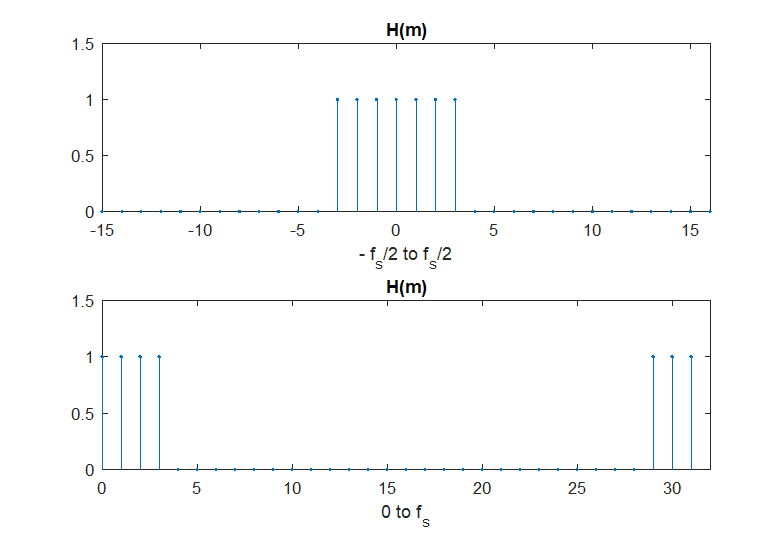
\includegraphics[width=0.6\linewidth]{graphics/windowmethod_1}
	\caption{Ideelt lavpasfilter set med kontinuert frekvensrespons og diskret frekvensrespons.}
	\label{fig:windowmethod_1}
\end{figure}

\begin{itemize}
	\item Der foretages en IDFT for at få filteret over i tidsdomænet.
	\begin{itemize}
		\item I tidsdomænet bliver responset repræsenteret som en sinc-funktion.
	\end{itemize}
	\item Sinc funktionen shiftes for at få peaket til at ligge midt i de valgte filterkoefficienter, da filterkoefficienterne skal være symmetriske for at få lineær fase.
	\begin{itemize}
		\item Den sidste sample fjernes for at shifte impulsresponsen.
	\end{itemize}
\end{itemize}

\begin{figure}[H]
	\centering
	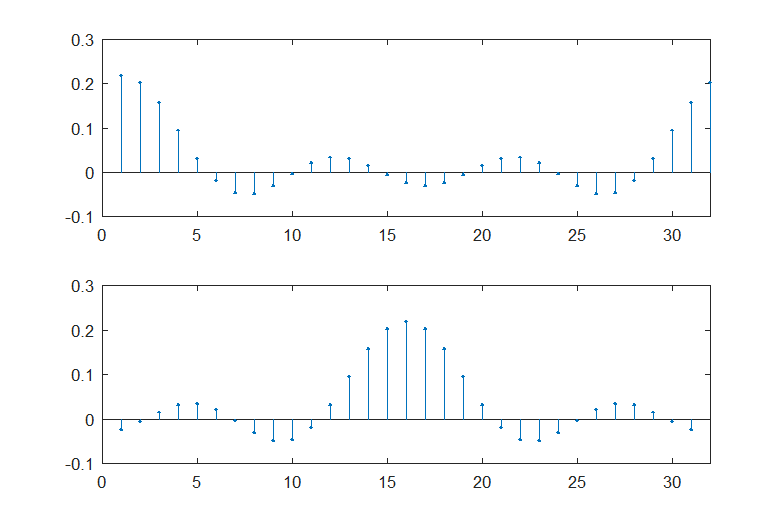
\includegraphics[width=0.6\linewidth]{graphics/windowmethod_2}
	\caption{IDFT af det diskrete respons efterfulgt af et symmetrisk respons der er blevet shiftet.}
	\label{fig:windowmethod_2}
\end{figure}

\begin{itemize}
	\item Et vindue ganges på for at udvælge betydende filterkoefficienter.
	\begin{itemize}
		\item Et vindue giver en kraftigere dæmpning.
	\end{itemize}
	\item Filteret kan trækkes over i frekvensdomænet med en DFT, for at validere at der gør som ønsket.
\end{itemize}

\begin{figure}[H]
	\centering
	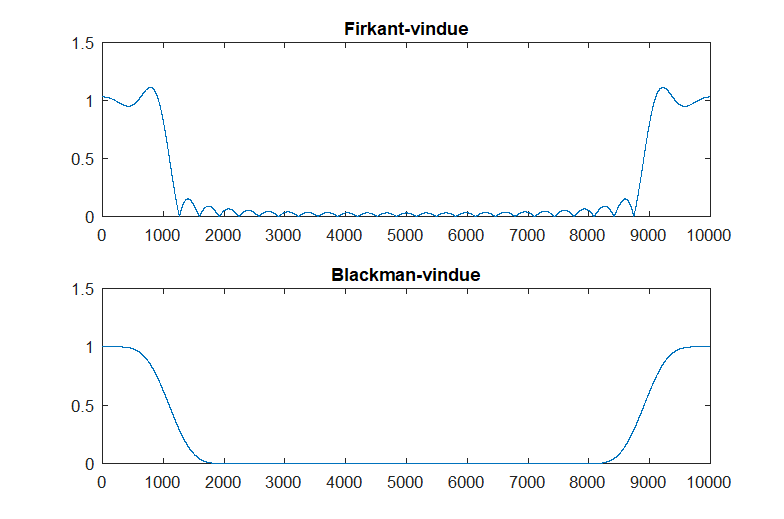
\includegraphics[width=0.6\linewidth]{graphics/windowmethod_3}
	\caption{Der anvendes DFT for at trække filteret over i frekvensdomænet for at validere det.}
	\label{fig:windowmethod_3}
\end{figure}

\subsection*{2 Typer af vinduer}
\begin{itemize}
	\item Et firkant vindue giver den skarpeste cut-off frekvens, men resultere i ripple på flankerne.
	\begin{itemize}
		\item Skyldes at firkanten repræsenteres som en sinc i frekvensdomænet, som foldes med den ideelle overføringsfunktion.
	\end{itemize}
	\item Et Blackman vindue giver en større dæmpning og mindre ripple, men derimod mindre skarpe flanker.
\end{itemize}


\end{document}
